
\subsection{Test Project Compilation and Execution}

Once we have generated a test project using TUG Wizard, in this
section we are going to describe how to compile and execute the
project, as well as how to check the results obtained from its
execution. This guide assumes that Qt Creator
(\url{https://qt-project.org/wiki/Category:Tools::QtCreator}) is being
used to open, compile, and deploy Qt-based projects.

%\setcounter{enumi}{4}
\begin{enumerate}

%
%%% 
%%
\item {\bf Step 0: Project structure.}\\
%
  The generated test project is composed of:
\begin{itemize}
\item a main project (represented by {\tt build\_all.pro} file in the
  figure below) that includes all test projects, and from which they
  can be compiled.

\item a folder including all test subprojects ({\tt tests} folder in
  the figure below).
\end{itemize}


\vspace{1ex}
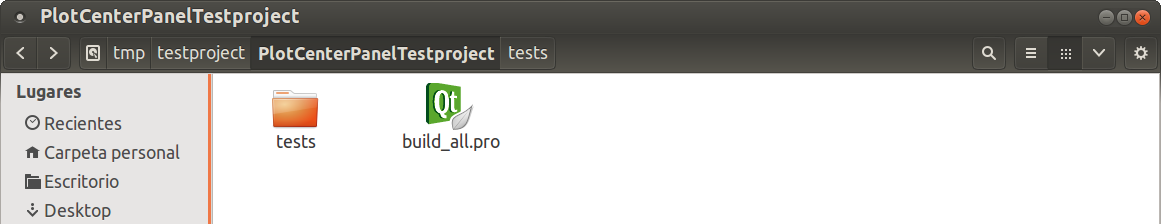
\includegraphics[width=.95\textwidth]{images/tug030a.png}
\vspace{3ex}

\newpage

Once opened the {\tt tests} folder, we can find:
\begin{itemize}

\item {\tt \_main} subproject including a class that inherits from the
  panel to test, and that includes a set of methods aimed at
  supporting the interaction with panel widgets.

\item all testsuites previously configured in TUG Wizard...

\item ...as well as the test projects from which they can be compiled
  and executed individually.
\end{itemize}

\vspace{1ex}
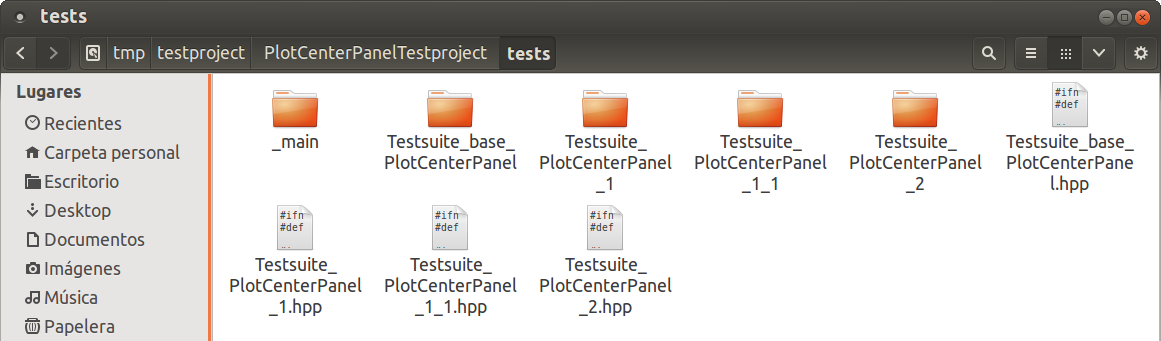
\includegraphics[width=.95\textwidth]{images/tug030b.png}
\vspace{3ex}

An snapshot of the {\_main} subproject is included below. The {\tt
  .pro} file can be opened using QtCreator to modify/compile/run the
project.

\vspace{1ex}
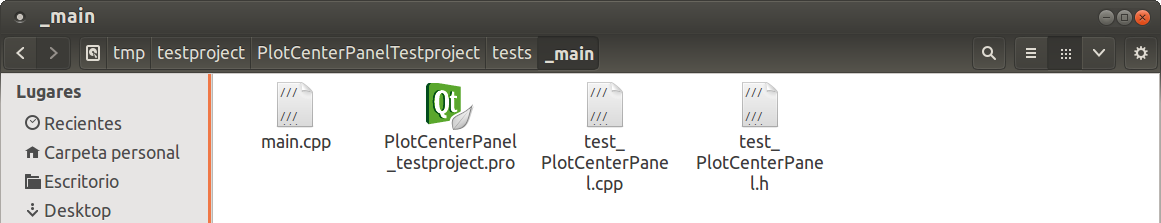
\includegraphics[width=.95\textwidth]{images/tug030c.png}
\vspace{3ex}

An snapshot of a testsuite subproject is included below.

\vspace{1ex}
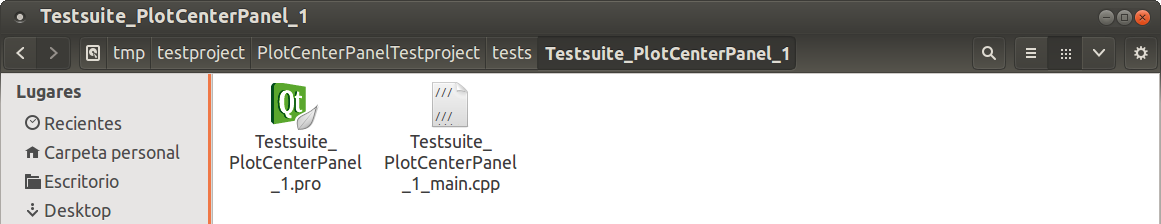
\includegraphics[width=.95\textwidth]{images/tug030d.png}
\vspace{3ex}

\newpage

%
%%% 
%%
\item {\bf Step 1: Open project.}\\
%
  Go to project folder. \\Double click
  {\tt build\_all.pro} file to open project in Qt Creator.


\vspace{1ex}
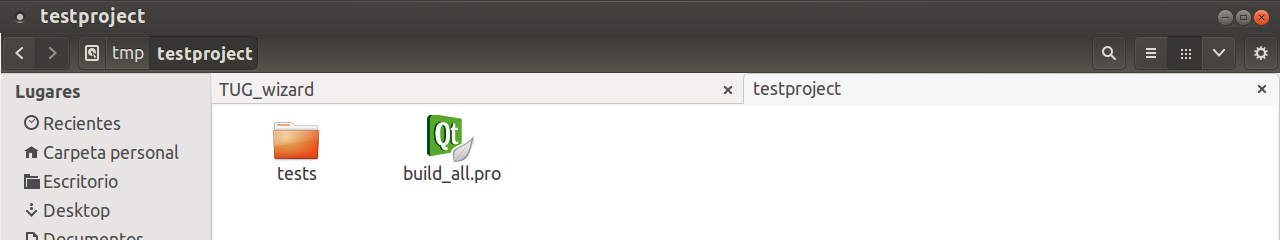
\includegraphics[width=.95\textwidth]{images/tug031.png}
\vspace{3ex}

%
%%% 
%%
\item {\bf Step 2: Configure project (i).}\\
%
  Once in Qt Creator, in
  \field{Configure Project} window, check only \field{Debug} version
  and click \field{Configure Project}.


\vspace{1ex}
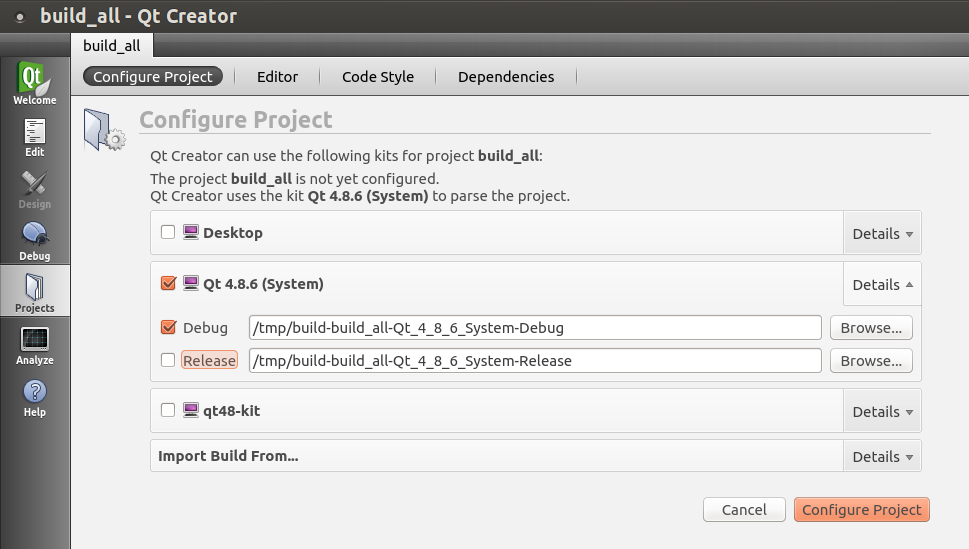
\includegraphics[width=.95\textwidth]{images/tug032.png}
\vspace{3ex}
\newpage

%
%%% 
%%
\item {\bf Step 3: Configure project (ii).}\\
%
  Go to \field{Projects}
  section in the tools bar at left. \\Uncheck \field{Shadow Build}.


\vspace{1ex}
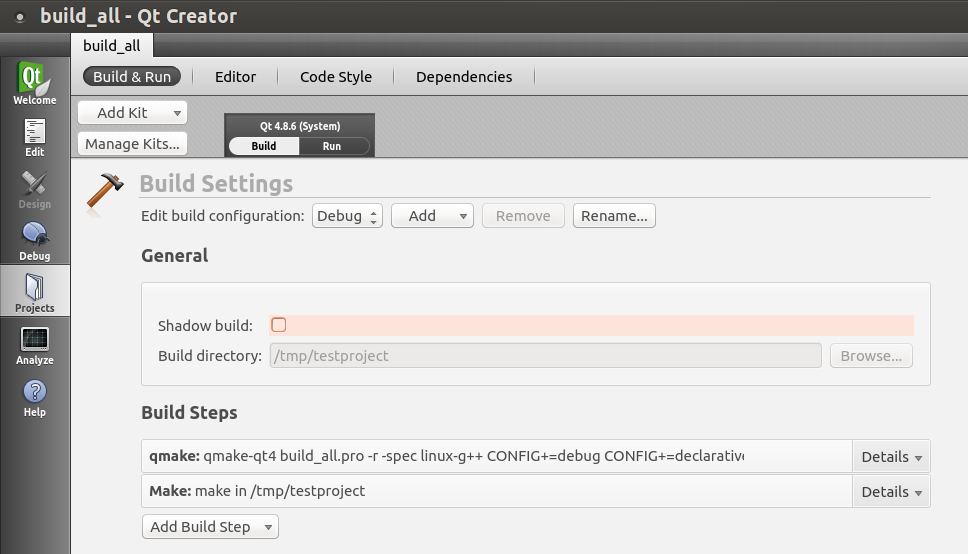
\includegraphics[width=.95\textwidth]{images/tug033.png}
\vspace{3ex}

%
%%% 
%%
\item {\bf Step 4: Project compilation.}\\
%
  Go to \field{Edit}
  section in the tools bar at left. \\Right click on
  \field{build\_all.pro} at the top of the projects list and then
  click \field{Rebuild}.

\vspace{1ex}
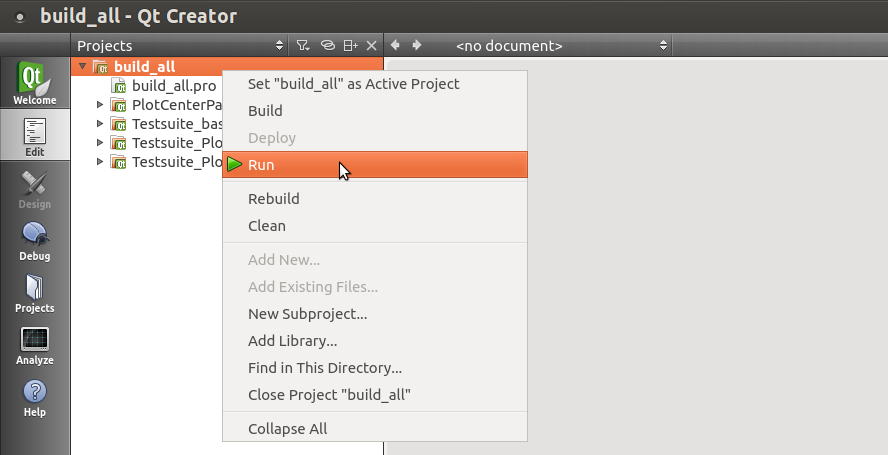
\includegraphics[width=.95\textwidth]{images/tug034.png}
\vspace{3ex}
\newpage

%
%%% 
%%
\item {\bf Step 5: Project execution.}\\
%
  Go to main project (it is
  placed the first in the project list), right click on it and then
  click \field{Run}.

\vspace{1ex}
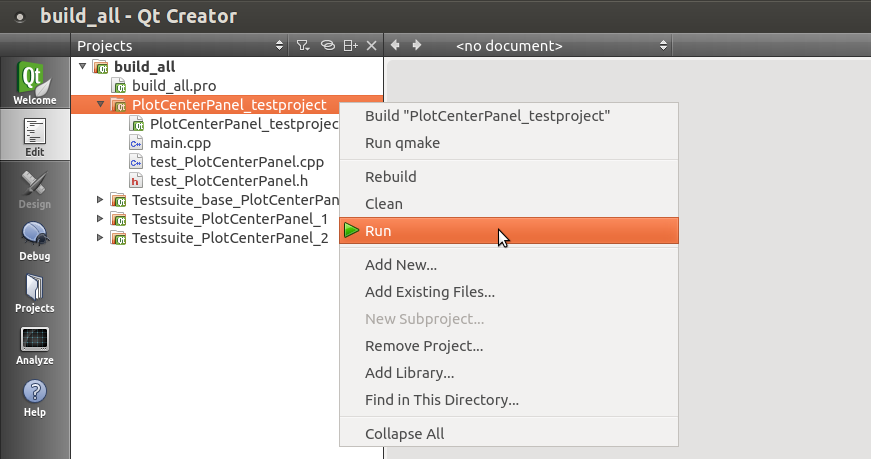
\includegraphics[width=.95\textwidth]{images/tug035.png}
\vspace{3ex}

%
%%% 
%%
\item {\bf Step 6: Check project output.}\\
%
  In the project folder, go to
  {\tt out} folder and open {\tt output.xml.html} file to see a
  summary of execution results.

\vspace{1ex}
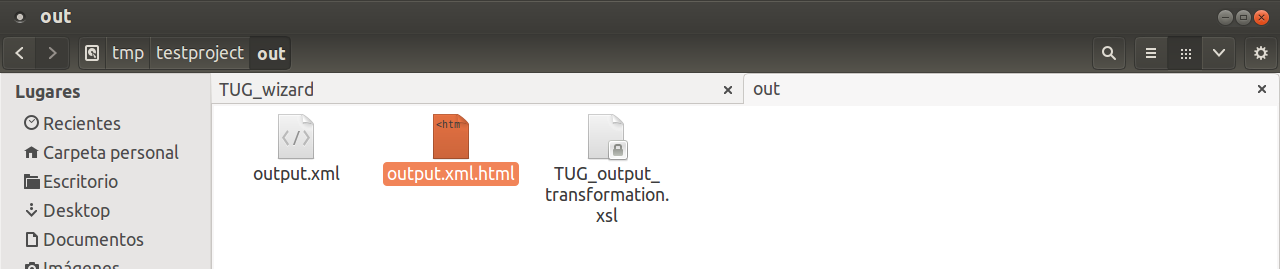
\includegraphics[width=.95\textwidth]{images/tug036.png}
\vspace{3ex}


\end{enumerate}



%%% Local variables:
%%% mode: latex
%%% TeX-master: "README.tex"
%%% ispell-local-dictionary: "american"
%%% coding: utf-8
%%% fill-column: 75
%%% TeX-parse-self: t
%%% TeX-auto-save: t
%%% End:
